\documentclass[pdflatex, a4paper,12pt]{article}
%\documentclass[a4paper,10pt]{scrartcl}

%some packages, mostly from malucrawl report
\usepackage[pdftex]{graphicx}
\usepackage[utf8x]{inputenc}
\usepackage{cite}
\usepackage{hyperref}
\usepackage{listings}
\usepackage{nomencl}
\usepackage{verbatim}
\usepackage{tabularx}
\usepackage{amsmath}

\providecommand{\e}[1]{\ensuremath{\times 10^{#1}}}

\begin{document}
\begin{center}
{\LARGE ELEC6032: Cryptography Coursework}\\[1em]

Author: Chris Orchard\\
\end{center}

TODO: an amount of intro?

\section{Q1}

Before attempting to decrypt the cipher, it was first necessary to transcribe
the hexadecimal string that formed the ciphertext into a format that was machine
readable. This was done by hand by copying the string into a binary hexadecimal
editor, and then comparing the two texts to ensure accuracy. In the process of
transcribing the ciphertext, it became obvious that there was a pattern in the
ciphertext aligned to to the byte boundaries and more likely aligned to a
multiple of four bytes, as there is a clearly visible pattern of similar bytes
in the columns of the cipher text, with the with in the provided image 28
characters. Upon performing autocorrelation of the ciphertext it was evident
that a likely key length was 32 bits, which correlates with the previous
observations. This however is one bit longer than the period of a degree 5 LFSR,
which the hint describes as the basis for the outer layer of encryption.

To break the LFSR cipher, a cracker was built using a C++ cryptographic library
\cite{_cryptographic-c---toolkit_????}, that iterated
through all possible states and characteristic functions of an LFSR and tried to
match the output to the given first two characters \verb+Ur+. This program
(included with this report as lfsr.cpp) successfully found an LFSR that provided
the appropriate plaintext, and the text derived is as follows:

\begin{quote}
\verbatiminput{fourth.tex}
\end{quote}

This does not look like the output of a possible alphanumeric cipher and in
fact it appears that every fourth character is incorrect, or at least is not an
alphanumeric character. It appears that an incorrect assumption has been made
about the key, that the key consists of 31 bits of LFSR output followed by a
single bit. Given the structure of ASCII it cannot be the case that the last bit
is incorrect, otherwise the output would look convincingly like alphanumeric text. 

Continuing to run with the assumption that all 31 bits of the LFSR are being
used, the next step is to find out where the last bit is placed. As the
implementation in \verb+lfsr.cpp+ computes the LFSR keystream on a byte by byte
basis, the first obvious place to try would be at the other end of the byte
meaning that the keystream would consist of 24 bits of LFSR, one arbitrary bit
(that is set to 0 in this case), followed by the last 7 bits of LFSR stream. The
output of this configuration is as follows:

\begin{quote}
\verbatiminput{decrypt.tex}
\end{quote}

The output of this stage now looks much more like the output of an alphanumeric
cipher. The next stage in decrypting the ciphertext is to apply frequency
analysis. Table (cite) shows the top 8 frequencies of letters in the English
language beside the top 8 frequencies in the ciphertext, derived from tools at
(cite).
\begin{center}
%\begin{tabularx}{0.8\textwidth}{cc|cc}
\begin{tabular}{cc|cc}
    \multicolumn{2}{c|}{English} & \multicolumn{2}{c}{Ciphertext} \\
    \hline
    Letter & Frequency(\%) & Letter & Frequency(\%) \\
    \hline
    E                & 12.7         & R      & 14.9  \\
    T                & 9.1          & G      & 8.6   \\
    A                & 8.2          & B      & 8.1   \\
    O                & 7.5          & F      & 7.0   \\
    I                & 7.0          & N      & 7.0   \\
    N                & 6.7          & V      & 6.6   \\
    S                & 6.3          & U      & 6.6   \\
    H                & 6.1          & A      & 6.4   \\
\end{tabular}
\end{center}

The frequencies indicate that the second stage cipher is probably a
monoalphabetic substitution cipher. To decrypt the cipher a second tool was
written in C++ \verb+monosubs.ccp+ that takes the substitution alphabet as
arguments and then displays the ciphertext and the plaintext. After replacing
the top 8 frequency characters in table (cite), it was then possible to do the
rest of the decryption by hand, resulting in the following output:

%\begin{minipage}{3in}
\begin{quote}
    \verbatiminput{cipherplain.tex}
\end{quote}
%\end{minipage}

The final substitution alphabet is as follows, shown as the arguments to the
substitution helper:

%\begin{quote}
\begin{verbatim}
./alpha n o p z r s t u v w q y j a b c d e f g h i x k l m
\end{verbatim}
%\end{quote}
By rearranging the unused characters to a more familiar order, it becomes
obvious that the second stage encryption is in fact ROT-13.

\section{Q2}

\subsection{Q2a}

Generator polynomials for Hamming codes must be primitive, as this ensures that
the Hamming distance of the generated cyclic code will be at least 3. 
\begin{align*}
f1(x) & = X^6 + X^3 + X^2 + X + 1\\
f2(x) & = X^6 + X^5 + X^4 + X^3 + 1\\
f3(x) & = X^6 + X^5 + X\\
f4(x) & = X^6 + X^5 + X^4 + X^3 + X^2 + X + 1\\
f5(x) & = X^6 + X + 1
\end{align*}

\begin{description}
    \item[f1(x)] Is not a primitive polynomial. 
    \item[f2(x)] Is not a primitive polynomial.
    \item[f3(x)] Is not a primitive polynomial.
    \item[f4(x)] Is not a primitive polynomial.
    \item[f5(x)] Is a primitive polynomial, as indicated by(cite).
\end{description}

\subsection{Q2b}



\subsection{Q2c}


\section{Q3}

This cipher takes form of a string of alphabetic characters with capitalisation
and some punctuation included. To start the process of decrypting the text, frequency
analysis was performed using the tool hosted at(cite). The top 8 results of
analysis are shown below.

\begin{center}
%\begin{tabularx}{0.8\textwidth}{cc|cc}
\begin{tabular}{cc|cc}
    \multicolumn{2}{c|}{English} & \multicolumn{2}{c}{Ciphertext} \\
    \hline
    Letter & Frequency(\%) & Letter & Frequency(\%) \\
    \hline
    E                & 12.7         & V      & 13.8  \\
    T                & 9.1          & R      & 9.2   \\
    A                & 8.2          & G      & 8.0   \\
    O                & 7.5          & L      & 7.6   \\
    I                & 7.0          & M      & 7.5   \\
    N                & 6.7          & H      & 6.3   \\
    S                & 6.3          & Z      & 6.3   \\
    H                & 6.1          & I      & 5.9   \\
\end{tabular}
\end{center}

The frequencies appear to match what would be expected for a simple
monoalphabetic substitution cipher. As in question one, the substitution helper
was used to solve the cipher.
Firstly the top 8 frequencies were swapped, and then the rest of the cipher was
completed by manual analysis. However, the letter frequencies for this cipher
do not match not those of English, as the cipher text contains multiple single capital
Rs which the frequency table shows should be substituted to T, but in English
can only correspond to the letter I. Eventually the plaintext was derived
primarily by solving the 2-3 letter words until the correct substitution for T
was found. The plaintext is as follows:

\begin{quote}
    Dear Sarah I am writing to apply for the programmer position advertised in the Times Union. as requested I am enclosing a completed job application, my certification my resume and three references The opportunity presented in this listing is very interesting and I believe that my strong technical experience and education will make me a very competitive candidate for this position The key strengths that I possess for success in this position include I have successfully designed, developed, and supported live use applications I strive for continued excellence I provide exceptional contributions to customer service for all customers With a BS degree in Computer Programming, I have a full understanding of the full life cycle of a software development project I also have experience in learning and excelling at new technologies as needed Please see my resume for additional information on my experience Thank you for your time and consideration I look forward to speaking with you about this employment opportunity You have now reached the end of this message 

\end{quote}    

The cipher for the text is as follows, and can be recognised as the Atbash
cipher as implemented for the Latin alphabet:

\begin{verbatim}
./alpha z y x w v u t s r q p o n m l k j i h g f e d c b a
\end{verbatim}

\section{Q4: Hacking the Mifare Classic}

\subsection{An Introduction to Mifare}

Mifare is a brand of RFID tag produced by NXP Semiconductor (formerly Philips)
aimed at low cost smartcards that can be easily distributed and used for
ingress/egress control and public transport systems. The Mifare Classic is the
simplest and until recently most widely used of the Mifare family(cite),
implementing a subset of the ISO/IEC 14443 Type A standard for contactless smart
cards, and a proprietary security protocol designed by NXP for which the details
are not published.

Between 2007 and 2009, a number of researchers reverse engineered the security
protocol and encryption method used in the Mifare Classic system, and found a
number of serious security vulnerabilities which the researchers used to
completely compromise the security of the cards. It was not only shown to be
possible to retrieve the data from the cards without the required key, but
possible to recover the key itself, and hence break the encryption. The attacks
demonstrated are possible with minimal computing resources, and can be performed
in sub-second times on a laptop in the case of the fastest attack. Researchers
have successfully used the attacks on the Mifare Classic system to gain unauthorised
access to access controlled buildings by cloning
cards\cite{digitalsecurityrun_mifare_2008}.

\subsection{The CRYPTO1 Cipher}

The encryption system used by Mifare Classic is known as CRYPTO1. The only
details published by NXP about CRYPTO1 is that it is a stream cipher with a
48 bit key. Nohl \& Plotz reverse engineered the system by analysing the
hardware of the Mifare Classic, using a microscope to take pictures of the
each layer of the silicon, polishing away each layer to reveal the next
\cite{nohl_reverse-engineering_????}. The
structure of the cipher was revealed using software to perform template
detection to detect individual gates, and then manual reconstructing the circuit
wiring. The cipher was revealed to be based on a 48 bit LFSR with the
characteristic function:

%TODO: insert characteristic function

This is a primitive polynomial, so the LFSR has the maximum state space of
(insert maths here). By analysing the protocol, it is also possible to derive
the structure of the random number generator used to generate the Nonce used by
the card in the authentication handshake. This is another LFSR, of 16 bits with
the characteristic function (some maths). The LFSR is linked to the clock, and
cycles through the state space every 0.6 seconds, and is reset to the 0 state on
power-on, a critical failure in the cryptographic design that allows for trivial
timing attacks on the cipher.

It is possible to reveal more details of the CRYPTO1 cipher by further
analysing the protocol. Garcia et al. manipulate the nonce and uid with a
hardware emulation of a Mifare Classic card, and find that the initial state of
the 48 bit LFSR is set to the secret key of the cardi\cite{garcia_dismantling_2008}.
Using a similar method it
is possible to derive the output function used to modify the output of the LFSR and
actually form the keystream. This was achieved by working out how to predict
then manipulate the output of the LFSR, revealing the function shown in Figure
\ref{fig:crypto1}.

\begin{figure}[htb]
\centering
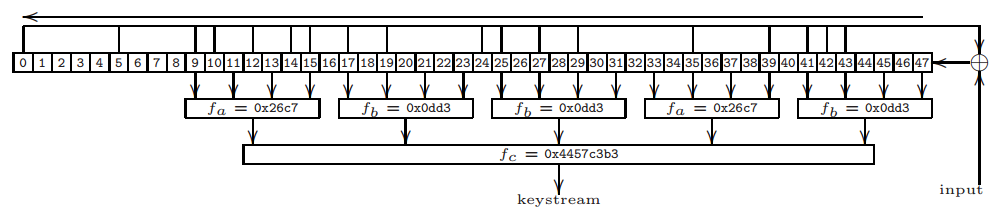
\includegraphics[width=\textwidth]{img/crypto1.png}
\caption{CRYPTO1 Cipher Description (reprinted from
\protect\cite{garcia_dismantling_2008})}
\label{fig:crypto1}
\end{figure}

\subsection{Breaking the Cipher}

The CRYPTO1 cipher can be broken in a number of ways, varying in complexity and
time and resources needed. Nohl \& Plotz identify that it is possible to brute
force the 48 bit key space, or generate rainbow tables for all possible secret
keys, that possibly can be used with timing manipulation to recover plaintext.
De Koning Gans et al. further this research by recovering keystream and hence
plaintext by capturing a successful transaction between a genuine card and
reader, and then using the timing attacks to generate a predictable nonce and
replay the captured data\cite{gans_practical_2008}. Because the request
specifying which block of data to
access is send in plaintext, it is possible to request known blocks and hence
recover the keystream. This allows data to be read (and write if a write
transaction is captured) from the secured storage without needing to posses the
secret key, although it might not be necessarily possible to retrieve all data.

Garcia et al. make considerably further progress using their Ghost device,
custom hardware that trivialises manipulating the nonce and UID sent by the card
by emulating a card, or manipulating the reader nonce by emulating a reader. Two
attacks on the cipher are specified. The first manipulates the UID and nonce
sent by the tag to reduce the search space for an LFSR state capable of
producing a given key space to 2**36 rather than 2**48. A table mapping all of
these possible LFSR states to produced keystreams must be produced, that is
approximately 1TB in size (although can be reused). 64 bits of keystream
recoverable from a failed authentication can then be used to recover the LFSR
state for that keystream. It is then possible to ``roll back'' the LFSR state to
find the secret key as the last bit of the LFSR is not used by the output
function. This method requires 4096 real authentication attempts to work, so
requires 2-14 minutes with a genuine reader. The second method is much more
advanced, but considerably quicker to execute. The output function of the cipher
is based solely on the odd outputs of the LFSR from 9-47, a pattern simple
enough to allow the search space of LFSR states to keystream to be split into
two 2**19 tables. Using this approach it is possible to use the inverse of the output
function to derive the LFSR state from 32/64 bits of keystream in less than a
second, which can then be rolled back to recover the secret key. Only one
authentication attempt is required for this attack, no prior preparation of
tables is required. This method of breaking the cipher is also effective for
recovering keys for other sectors, as the authentication request can be
decrypted by the first key. The tag nonce for the next sector is encrypted, but
can be guessed by exploiting the re-use of the key-stream for parity bits. 

\subsection{Conclusions}

The cryptographic system used in Mifare Classic RFID cards, CRYPTO1 is very
weak with a number of serious design flaws allowing the entire cryptographic
system to be broken with little hardware in a trivial amount of time. Many of
these design issues could have been possibly avoided if NXP had shared the specification of
CRYPTO1 at any point, so it could be rigorously tested by the community before
it reached widespread use. Instead Mifare Classic relies on security through
obscurity, an approach that did not work, in part thanks to the simplicity of
CRYPTO1. This simplicity can be in part be put down to the compromise made by
the designers of Mifare Classic between the security of the system and the
requirement that it should draw sufficiently small amounts of power to be
powered by induction from the reader. The large feature size and lack of
anti-tampering measures that allowed the
physical structure to be analysed could also be related to compromising to
reduce the cost of the cards.

The Mifare Classic system is still in use at the University Of Southampton for
access control and public transport, and if a Ghost-like device were to be
re-created it would be trivial to clone cards for access, or modify cards for
access to transport. The Mifare Classic system was previously also used for the
Oyster contactless system run by Transport for London but has been replaced
with a more secure version, primarily because of the security concerns
highlighted above.

\bibliographystyle{IEEEtran}
%\bibliography{irp-report,rfc,i-d}{}
\bibliography{crypto}{}

\end{document}
